\documentclass[11pt]{article}
\usepackage[margin=1in]{geometry}
\usepackage{amsmath,amssymb,amsthm,mathtools}
\usepackage{graphicx}
\usepackage{microtype}
\usepackage[hidelinks]{hyperref}

\newtheorem{theorem}{Theorem}[section]
\newtheorem{lemma}[theorem]{Lemma}
\newtheorem{corollary}[theorem]{Corollary}
\theoremstyle{remark}
\newtheorem{remark}[theorem]{Remark}

\newcommand{\R}{\mathbb{R}}
\newcommand{\E}{\mathbb{E}}
\newcommand{\ffbox}{\mathbin{\boxplus_{2}}}
\newcommand{\freebox}{\mathbin{\boxplus}}
\newcommand{\pos}[1]{\left(#1\right)_{+}}

\title{The degree-two case of the finite-free\\fourth-order comparison}
\author{Autonomous proof-discovery packet for arXiv:2602.10373}
\date{11 August 2026}

\begin{document}
\maketitle

\begin{abstract}
Hein\"avaara conjectures that the empirical root law of a finite free
additive convolution is below the corresponding free convolution for every
test function with nonnegative fourth derivative.  We prove the conjecture
for arbitrary monic real-rooted quadratic polynomials.  The key observation
is a general extremal principle: among symmetric compactly supported laws of
fixed variance, the symmetric two-point law minimizes every fourth-order
convex test.  Its proof is a direct Jensen argument applied to the square of
the random variable.
\end{abstract}

\section{Source problem}

Let $p$ and $q$ be monic real-rooted polynomials of the same degree $d$,
and let $\mu_p,\mu_q$ denote their empirical root measures.  The finite free
additive convolution $p\boxplus_d q$ is again real-rooted.  Conjecture~5.2 of
Hein\"avaara~\cite{Heinavaara2026} asks whether
\begin{equation}\label{eq:source-conjecture}
 \frac1d\sum_{x:(p\boxplus_d q)(x)=0} f(x)
 \leq \int_{\R} f(t)\,d(\mu_p\freebox\mu_q)(t)
\end{equation}
for every $f\in C^4(\R)$ satisfying $f^{(4)}\geq0$.

The exact source passage is reproduced in Figure~\ref{fig:source}.  It also
records the weaker even-moment question that motivated the conjecture.

\begin{figure}[ht]
  \centering
  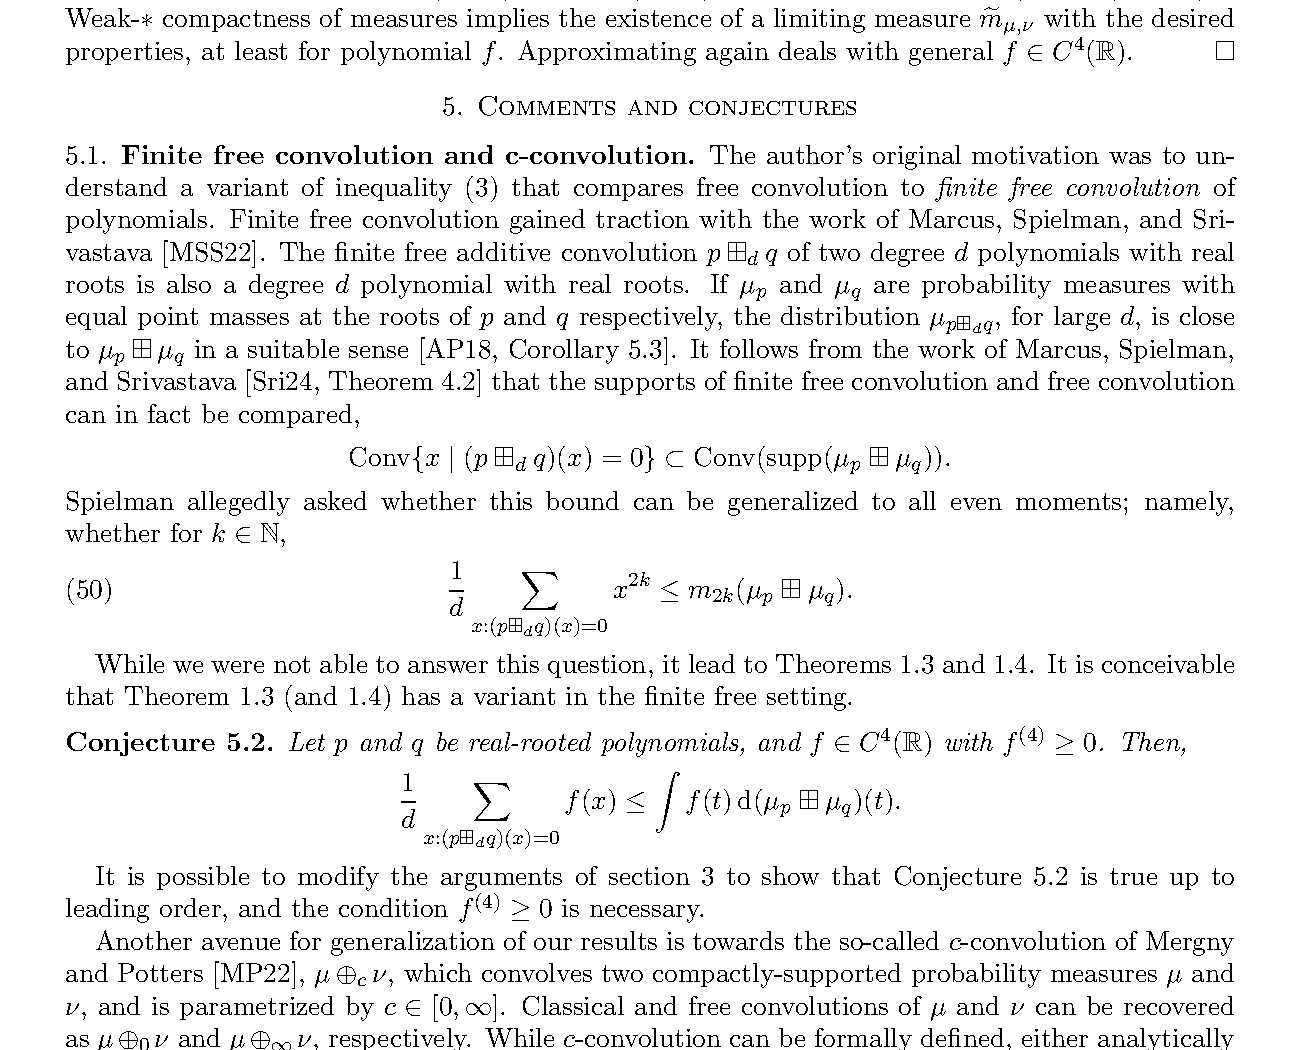
\includegraphics[width=\textwidth]{figures/conjecture_5_2_crop.png}
  \caption{Conjecture~5.2 and its context on page 16 of
  arXiv:2602.10373.}
  \label{fig:source}
\end{figure}

\section{Result}

\begin{theorem}[Quadratic finite-free comparison]\label{thm:main}
Let $p,q$ be arbitrary monic real-rooted quadratic polynomials.  Then
\eqref{eq:source-conjecture} holds with $d=2$ for every
$f\in C^4(\R)$ with $f^{(4)}\geq0$.
\end{theorem}

In the notation for the fourth-order order introduced in the source, this is
the assertion
\[
 \mu_{p\ffbox q}\prec_4 \mu_p\freebox\mu_q
 \qquad (\deg p=\deg q=2).
\]
The result includes repeated roots.  It is exact, not asymptotic, and the test
class is the full class appearing in the conjecture.

\section{Idea of the proof}

Write the roots of $p$ as $m\pm\alpha$ and those of $q$ as
$n\pm\beta$.  The finite-free coefficient formula collapses to
\[
 (p\ffbox q)(x)=(x-m-n)^2-(\alpha^2+\beta^2).
\]
Thus, after removing the common center $m+n$, the finite root law is exactly
the symmetric two-point law at $\pm r$, where
$r^2=\alpha^2+\beta^2$.

The centered free convolution is the law of $Z=\alpha U+\beta V$, with
$U,V$ freely independent symmetric Bernoulli variables.  It is symmetric and
$\E Z^2=r^2$.  Fourth-order convex comparison is generated by the cubic
stop-loss kernels $\pos{x-t}^3$.  For $t\geq0$, symmetry gives
\[
 \E\pos{Z-t}^3=\frac12\E\pos{|Z|-t}^3.
\]
The map $v\mapsto\pos{\sqrt v-t}^3$ is convex, so Jensen compares the
right-hand side with its value at $\E Z^2=r^2$.  This is precisely the cubic
stop-loss transform of the two-point law.  Symmetry handles negative $t$,
and Taylor's integral remainder handles an arbitrary $f$.

\section{A fourth-order extremal lemma}

\begin{lemma}\label{lem:extremal}
Let $Z$ be a compactly supported symmetric real random variable and let
$r^2=\E Z^2$.  Let $Y$ take the two values $-r,r$ with probability $1/2$
each.  Then for every $f\in C^4(\R)$ with $f^{(4)}\geq0$,
\[
 \E f(Y)\leq \E f(Z).
\]
\end{lemma}

\begin{proof}
For $t\in\R$, put
\[
 D(t)=\E\pos{Z-t}^3-\E\pos{Y-t}^3.
\]
First suppose $t\geq0$.  Define on $[0,\infty)$
\[
 g_t(v)=\pos{\sqrt v-t}^3.
\]
It vanishes on $[0,t^2]$.  On $(t^2,\infty)$, direct differentiation gives
\[
 g_t''(v)=\frac{3(v-t^2)}{4v^{3/2}}\geq0.
\]
The value and first derivative glue continuously to zero at $v=t^2$;
hence $g_t$ is convex on all of $[0,\infty)$.  By symmetry and Jensen's
inequality,
\begin{align*}
 \E\pos{Z-t}^3
 &=\frac12\E\pos{|Z|-t}^3
  =\frac12\E g_t(Z^2)\\
 &\geq\frac12 g_t(\E Z^2)
  =\frac12\pos{r-t}^3
  =\E\pos{Y-t}^3.
\end{align*}
Thus $D(t)\geq0$ for $t\geq0$.

For a symmetric random variable $W$, symmetry and the elementary identity
\[
 \pos{t-W}^3-\pos{W-t}^3=(t-W)^3
\]
give
\[
 \E\pos{W+t}^3
 =\E\pos{W-t}^3+\E(t-W)^3.
\]
The variables $Z$ and $Y$ have the same moments through order three:
both are symmetric, centered, and have second moment $r^2$.  Subtracting the
last display for $W=Z$ and $W=Y$ yields $D(-t)=D(t)$.  Therefore
$D(t)\geq0$ for every real $t$.

Choose a compact interval $[a,b]$ containing the supports of $Z$ and $Y$.
For $x\in[a,b]$, Taylor's formula with integral remainder gives
\[
 f(x)=P_3(x)+\frac16\int_a^b\pos{x-t}^3 f^{(4)}(t)\,dt,
\]
where $P_3$ is a polynomial of degree at most three.  The expectations of
$P_3$ agree for $Z$ and $Y$.  Hence Fubini's theorem gives
\[
 \E f(Z)-\E f(Y)
 =\frac16\int_a^b D(t)f^{(4)}(t)\,dt\geq0.
\]
\end{proof}

\section{Finite and free quadratic convolutions}

\begin{lemma}\label{lem:finite}
Suppose
\[
 p(x)=(x-m)^2-\alpha^2,
 \qquad q(x)=(x-n)^2-\beta^2,
 \qquad \alpha,\beta\geq0.
\]
Then
\[
 (p\ffbox q)(x)=(x-m-n)^2-\alpha^2-\beta^2.
\]
\end{lemma}

\begin{proof}
Write $p=x^2-a_1x+a_2$ and $q=x^2-b_1x+b_2$.  Thus
\[
 a_1=2m,\quad a_2=m^2-\alpha^2,
 \qquad b_1=2n,\quad b_2=n^2-\beta^2.
\]
The degree-two specialization of the finite-free coefficient formula
of Marcus--Spielman--Srivastava~\cite{MSS2022} is
\[
 p\ffbox q=x^2-(a_1+b_1)x+
 \left(a_2+b_2+\frac12a_1b_1\right).
\]
Substitution gives the claimed expression.
\end{proof}

\begin{lemma}\label{lem:free}
With the notation of Lemma~\ref{lem:finite}, the free convolution
$\mu_p\freebox\mu_q$, translated by $-(m+n)$, is symmetric and has second
moment $\alpha^2+\beta^2$.
\end{lemma}

\begin{proof}
Let $U,V$ be freely independent symmetric Bernoulli variables, each taking
the values $-1,1$ with equal probability.  The desired centered law is the
law of
\[
 Z=\alpha U+\beta V.
\]
The trace-preserving sign change $(U,V)\mapsto(-U,-V)$ in the free product
shows that $Z$ is symmetric.  Also, freeness and centering give
$\E(UV)=\E(VU)=0$, while $U^2=V^2=1$.  Therefore
\[
 \E Z^2=\alpha^2+\beta^2.
\]
\end{proof}

\begin{proof}[Proof of Theorem~\ref{thm:main}]
Every monic real-rooted quadratic admits the parametrization in
Lemma~\ref{lem:finite}.  Put $r^2=\alpha^2+\beta^2$.  That lemma identifies
the centered empirical root law of $p\ffbox q$ with the symmetric two-point
law at $\pm r$.  Lemma~\ref{lem:free} identifies the centered free
convolution as a symmetric law with the same second moment.  Apply
Lemma~\ref{lem:extremal}, then translate both laws back by $m+n$.
\end{proof}

\begin{corollary}[Even moments in degree two]
For every integer $k\geq1$,
\[
 \frac12\sum_{x:(p\ffbox q)(x)=0}x^{2k}
 \leq m_{2k}(\mu_p\freebox\mu_q).
\]
\end{corollary}

\begin{proof}
For $k=1$ there is equality by the first-three-moment calculation.  For
$k\geq2$, take $f(x)=x^{2k}$ in Theorem~\ref{thm:main}; its fourth
derivative is nonnegative on $\R$.
\end{proof}

\section{Verification, scope, and upgrade attempts}

The symbolic verifier in \texttt{code/verify\_degree\_two.py} checks both
algebraic identities on which the proof rests: the finite-free quadratic
coefficient formula and
\[
 \frac{d^2}{dv^2}(\sqrt v-t)^3
 =\frac{3(v-t^2)}{4v^{3/2}}.
\]
The exploratory attempt also performed exact rational moment searches and
Haar-matrix stop-loss searches; none is used in the proof.

Six materially different upgrade routes were pursued.  The successful route
above emerged after exact even-moment and stop-loss searches.  For symmetric
cubics the finite convolution has roots $0,\pm\sqrt{\alpha^2+\beta^2}$,
so its squared modulus is no longer constant and the Jensen extremality
breaks.  Existing finite-free majorization compares finite convolutions to
other finite convolutions rather than to the free limit.  Finally, the
Mergny--Potters $c$-interpolation yields explicit hypergeometric laws only in
special cases and did not provide a sign-definite stop-loss derivative.

Thus the packet settles the source conjecture completely in degree two but
does not claim the general-degree result.  Bounded exact-phrase and concept
searches through 11 August 2026 found the source conjecture, finite-free
cumulant papers, and the standard majorization results, but no prior statement
of this quadratic fourth-order comparison.  This is a novelty check, not a
guarantee of novelty.

\begin{thebibliography}{9}

\bibitem{Heinavaara2026}
O.~Hein\"avaara,
\emph{Convolution comparison measures},
arXiv:2602.10373, 2026.

\bibitem{MSS2022}
A.~W. Marcus, D.~A. Spielman, and N.~Srivastava,
\emph{Finite free convolutions of polynomials},
Probab. Theory Related Fields \textbf{182} (2022), 807--848;
arXiv:1504.00350.

\bibitem{NicaSpeicher2006}
A.~Nica and R.~Speicher,
\emph{Lectures on the Combinatorics of Free Probability},
London Math. Soc. Lecture Note Ser. 335, Cambridge Univ. Press, 2006.

\end{thebibliography}

\end{document}

